\section{Optimizing Cooling of Various Stations}
\label{sec:efficiency}

The fan delivered the most cooling per kilowatt-hour in all 36 modeled venue and weather combinations. It also led per dollar of equipment purchase price in 25 cases. The larger evaporative cooler led in the other 11.

We measured cooling as the reduction in Standard Effective Temperature (SET) from the no-device case at the same venue and under the same weather. We divided this reduction by electricity used during the modeled hour and by equipment purchase price. The 36 cases cover four venue types in Dallas, Boston, and Phoenix, each under peak-temperature, hot-humid, and hot-dry conditions.

\begin{figure}[H]
    \centering
    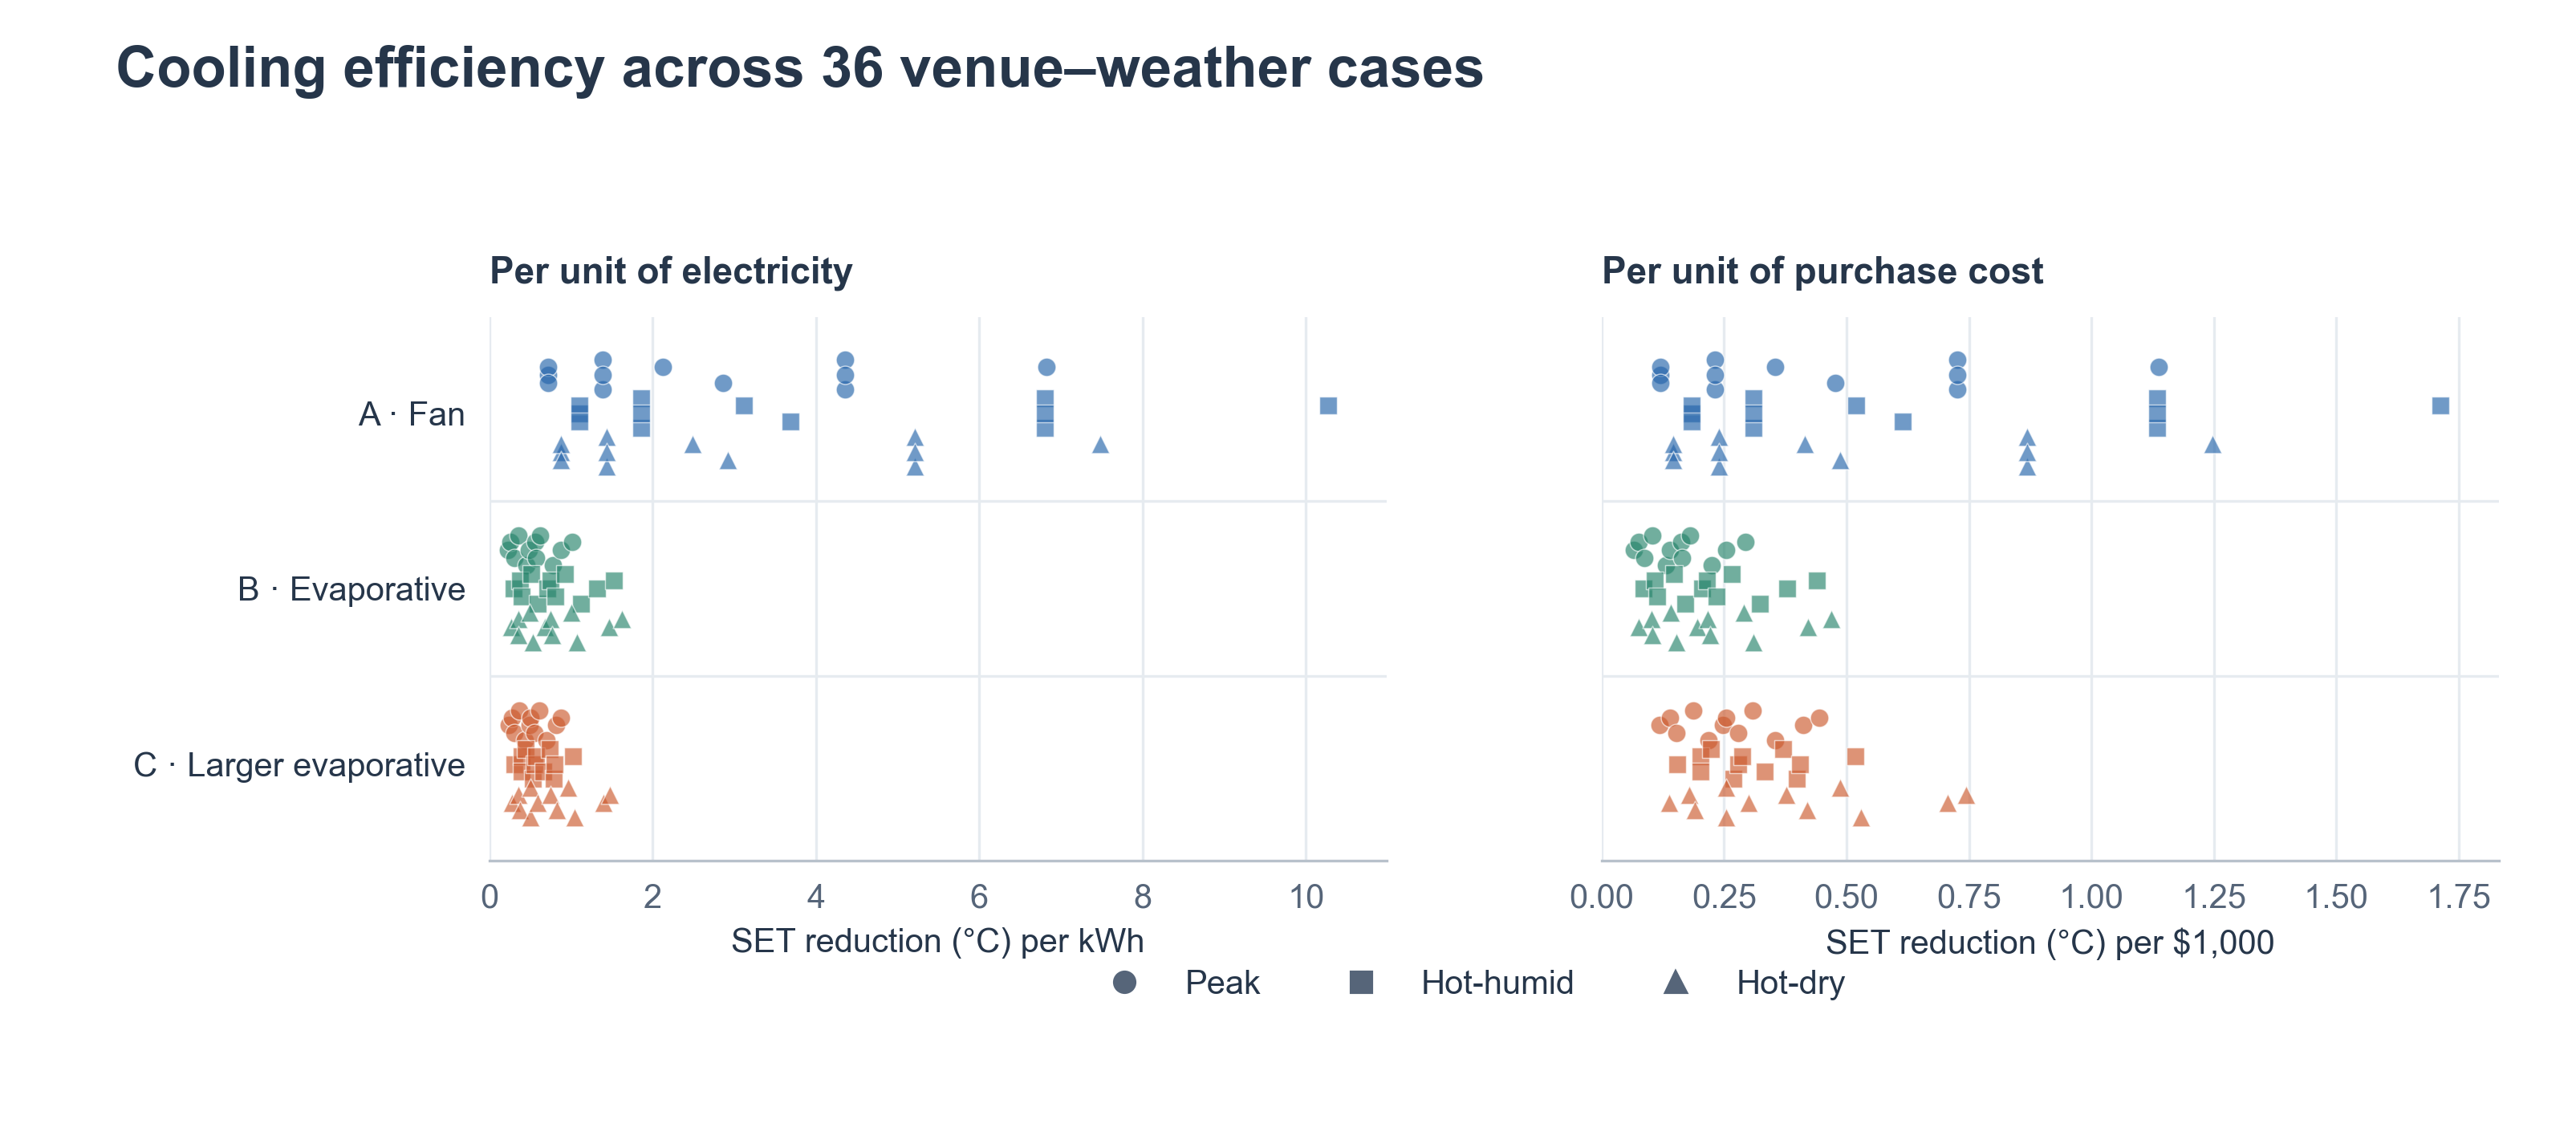
\includegraphics[width=0.94\linewidth]{Images/F6_efficiency_all_cases.png}
    \caption{Cooling per kWh and per \$1,000 of equipment purchase price across all 36 cases.}
    \label{fig:efficiency}
\end{figure}

The fan delivered 1.14 to 9.59 times the cooling per kWh of the more efficient evaporative cooler in the same case. The advantage was smallest at the Dallas rail platform in the hot-dry scenario and largest under the Boston airport canopy in the hot-humid scenario.

\subsection{Adapting the Bus-Shelter Model to Rail}
For Dallas, the modeled rail platform uses 5.81 kg/s of dry-air exchange and a baseline passenger airspeed of 1.40 m/s, compared with 2.18 kg/s and 0.93 m/s at the bus shelter. These are scenario estimates based on different equivalent openings and sheltering factors. We hold weather, equipment, and exposure duration fixed within the city so the comparison reflects the two airflow assumptions.

The higher outdoor exchange dilutes the evaporative cooler's supply air. The higher rail baseline airspeed also leaves less scope for a fan modeled at the same operating airspeed at both sites. The peak-hour figures below show both effects. Using separate airflow assumptions lets the model compare the two layouts. Field measurements would be needed to test its accuracy at either location.

\subsection{Purchase Price and Peak Hour Cooling}

Option C led per purchase dollar in ten Dallas cases and at the Phoenix rail platform in hot-dry weather. At the Dallas rail platform it led in all three scenarios. The fan led throughout Boston. These comparisons use upfront equipment price.

During peak heat, the Dallas bus shelter fan reduced SET by 0.53\ensuremath{^{\circ}\mathrm{C}} using 0.25 kWh, compared with 1.75\ensuremath{^{\circ}\mathrm{C}} using 2.50 kWh for the larger cooler. At the Dallas rail platform, the same devices reduced SET by 0.18\ensuremath{^{\circ}\mathrm{C}} and 1.38\ensuremath{^{\circ}\mathrm{C}}, respectively. At both sites the extra 2.25 kWh delivered about 1.2\ensuremath{^{\circ}\mathrm{C}} more cooling.

\begin{figure}[H]
    \centering
    \begin{subfigure}[t]{0.43\textwidth}
        \centering
        \vspace{0pt}
        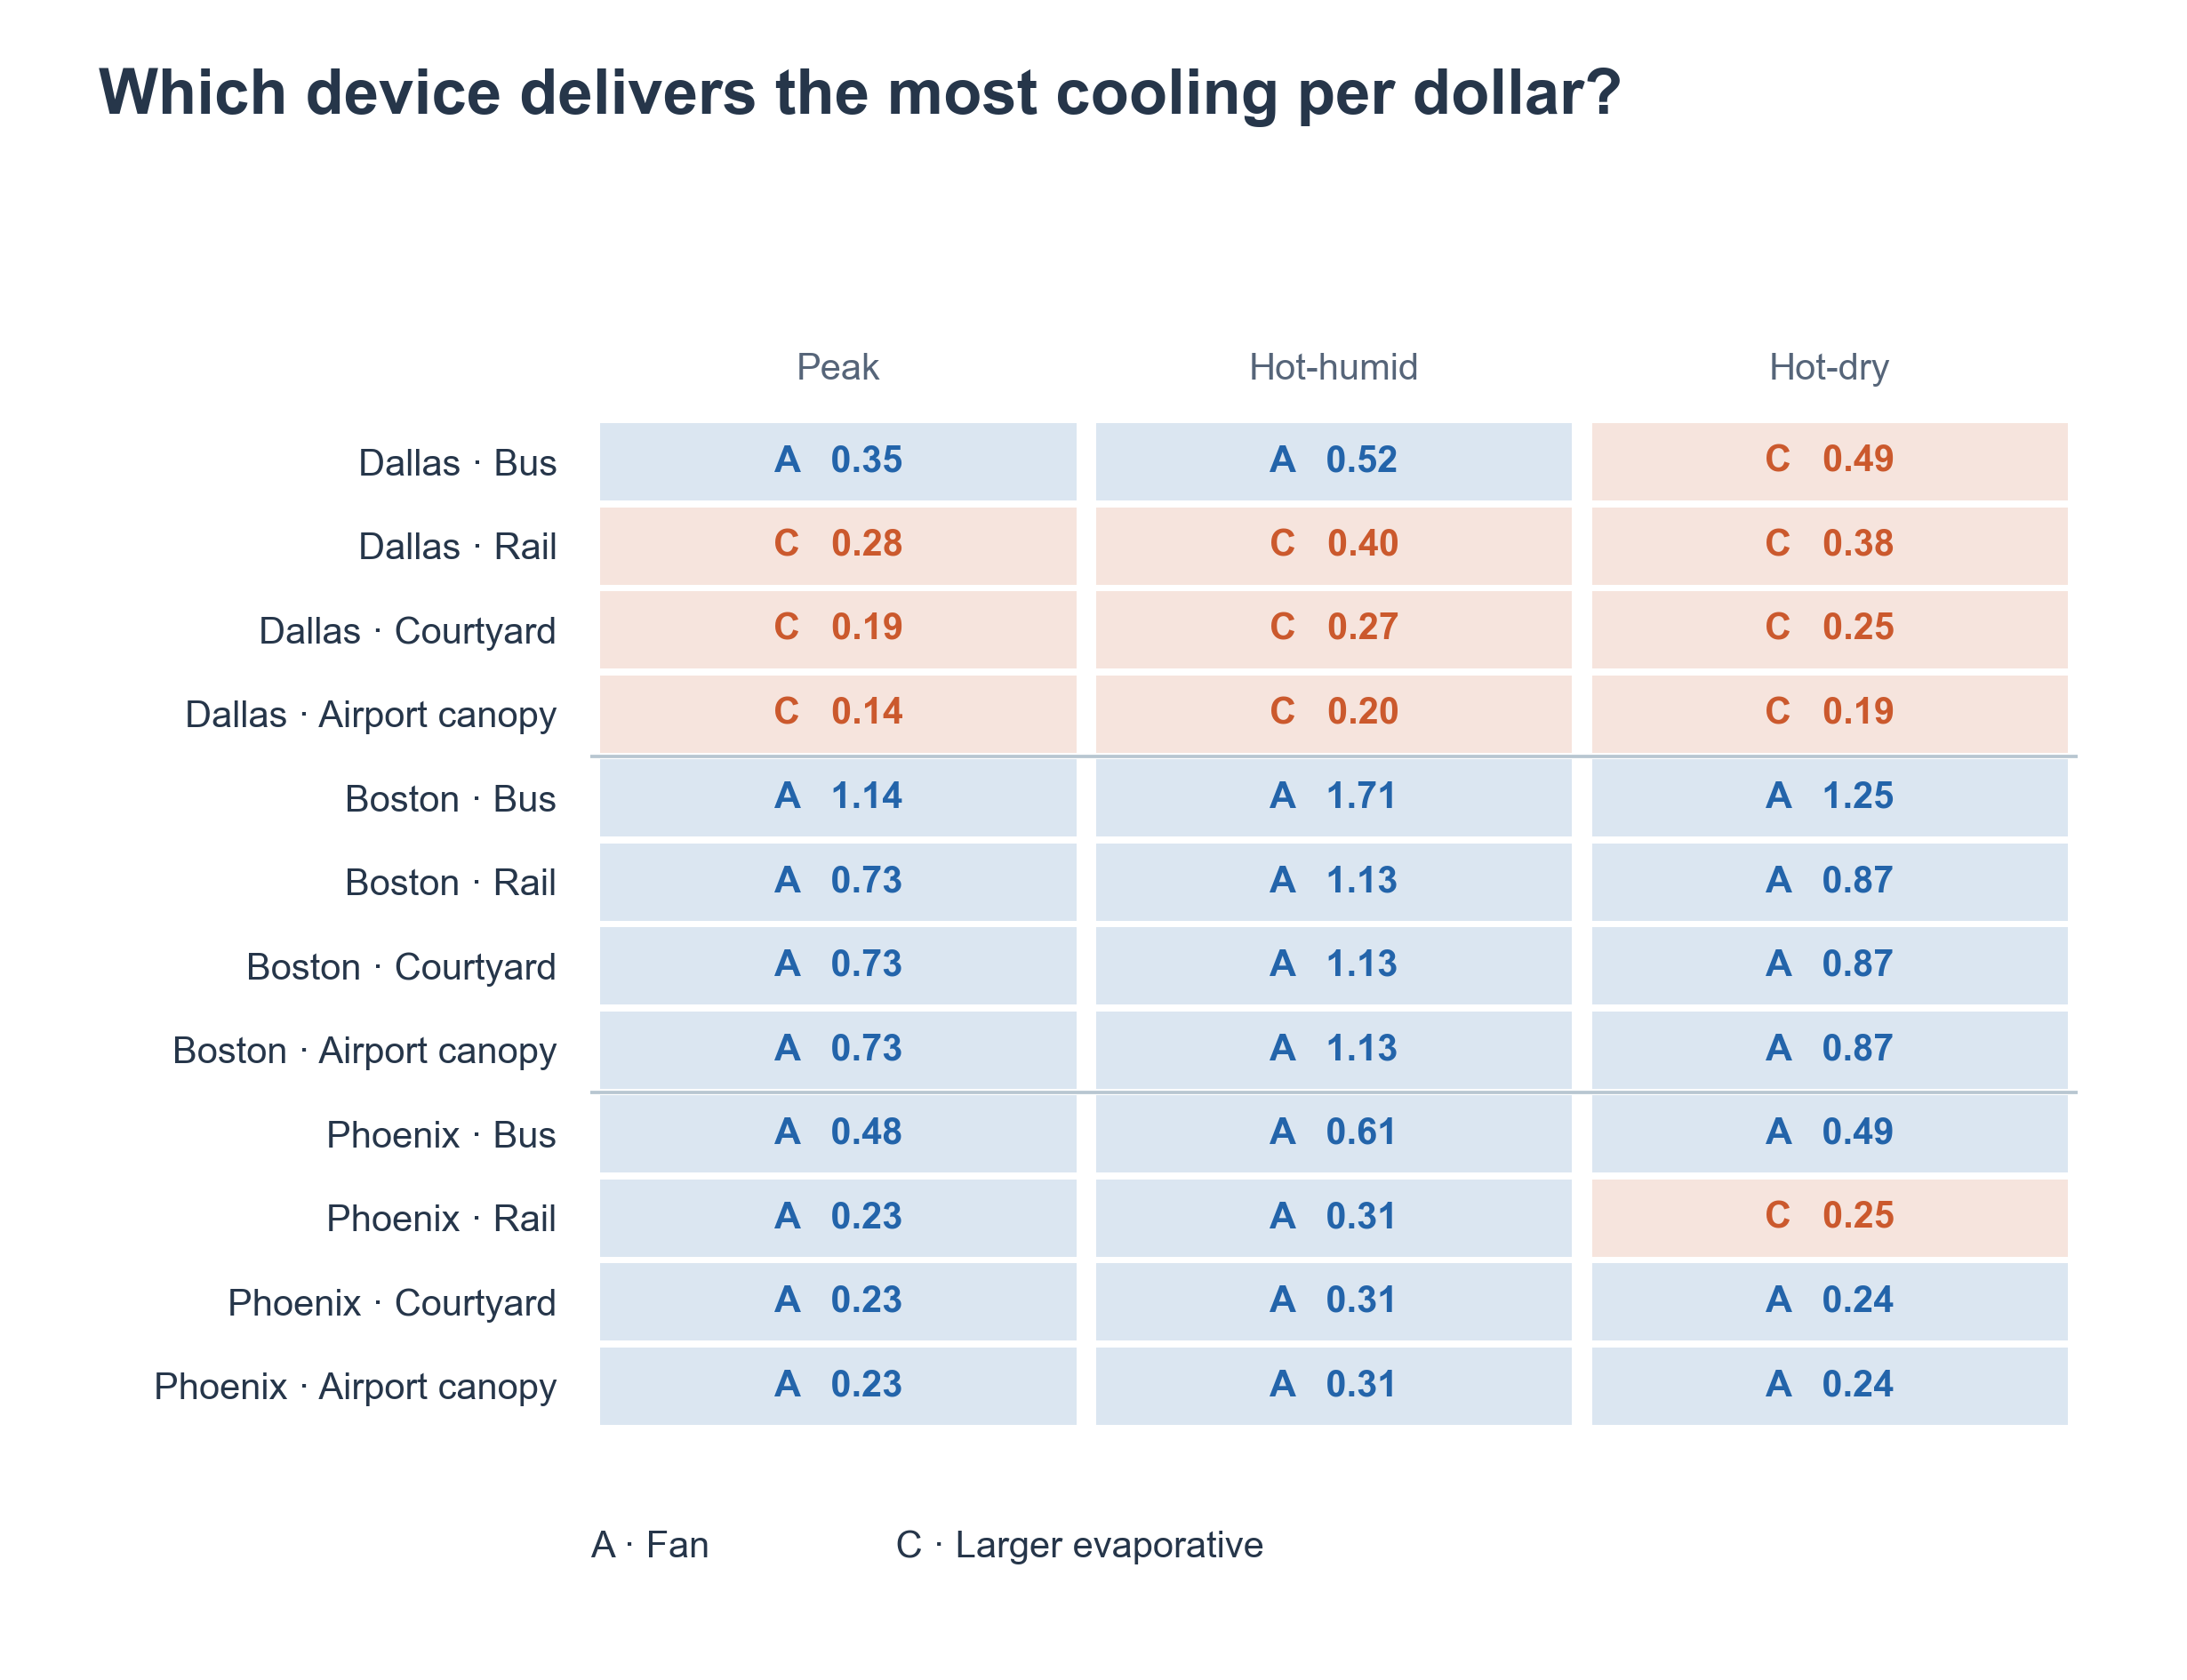
\includegraphics[width=\linewidth]{Images/F9_purchase_efficiency_winners.png}
        \caption{Purchase-price efficiency leader by venue and weather. The number is SET reduction in degrees Celsius per \$1,000.}
        \label{fig:purchase-efficiency}
    \end{subfigure}
    \hfill
    \begin{subfigure}[t]{0.54\textwidth}
        \centering
        \vspace{0pt}
        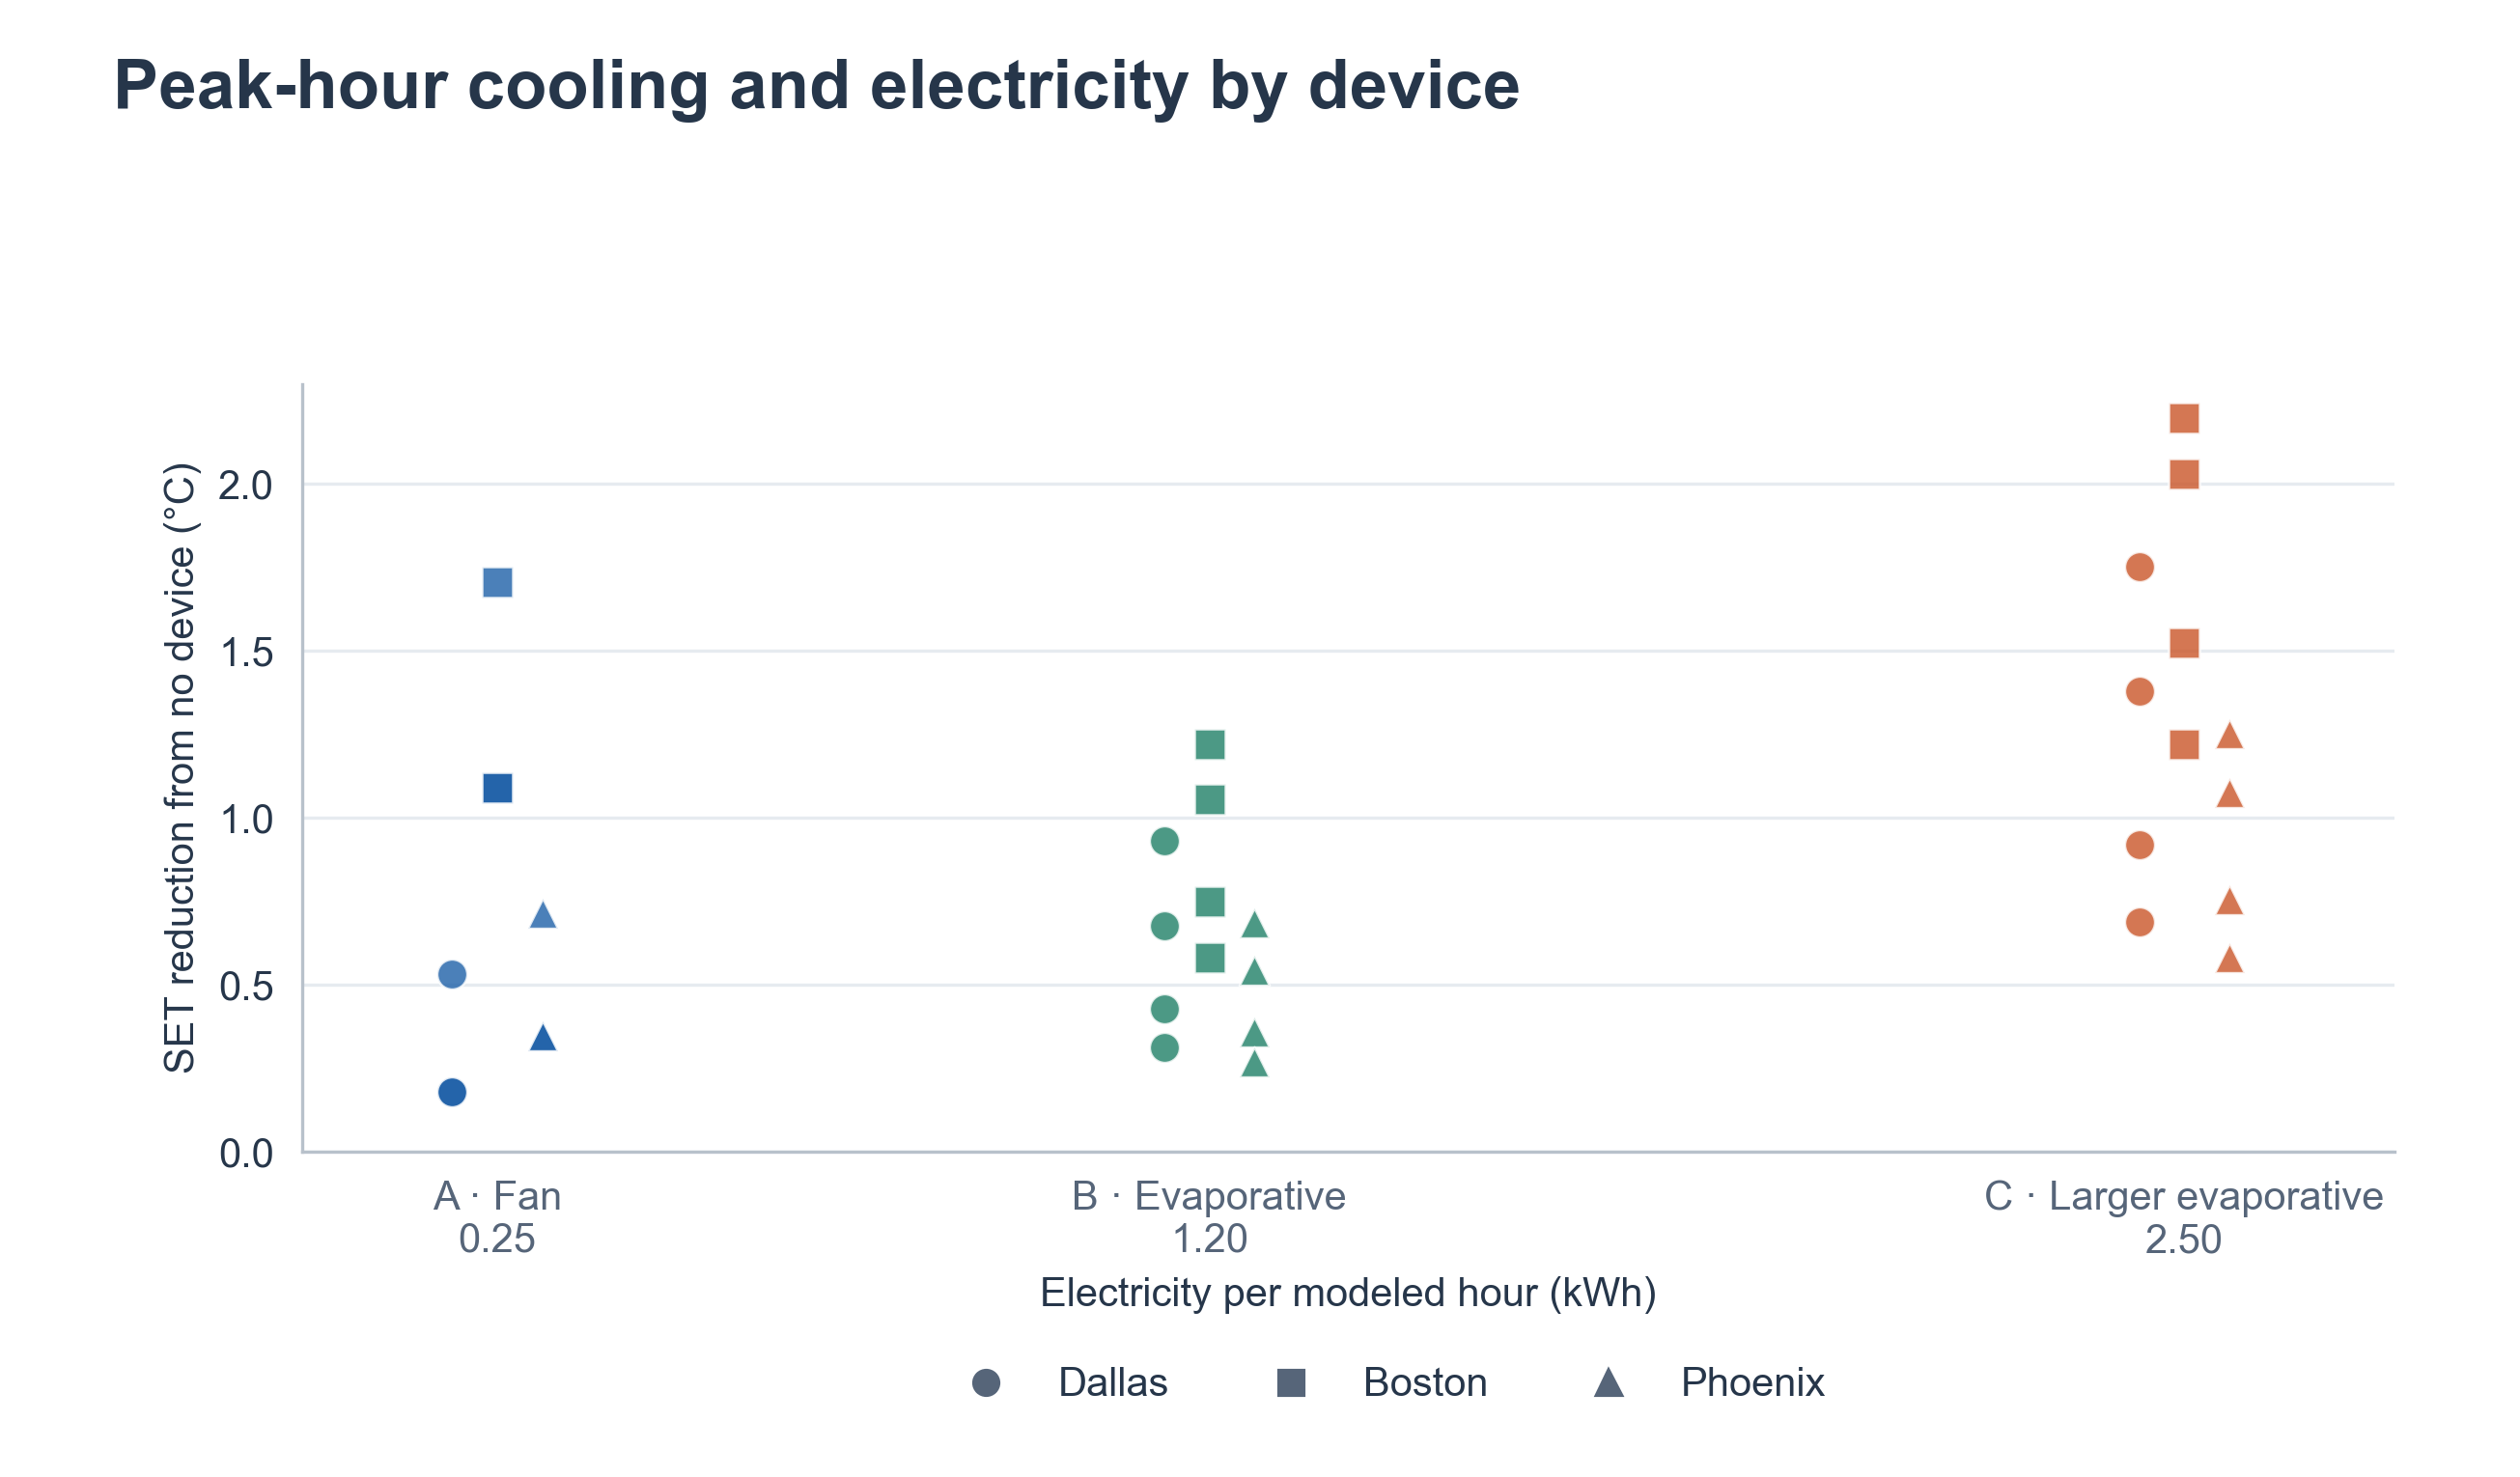
\includegraphics[width=\linewidth]{Images/F10_peak_cooling_electricity.png}
        \caption{Peak-hour SET reduction and electricity use. Each device has the same electricity use at all venues in the one-hour comparison.}
        \label{fig:peak-electricity}
    \end{subfigure}
    \caption{Purchase-price efficiency and peak-hour electricity tradeoffs.}
    \label{fig:purchase-and-peak}
\end{figure}

\subsection{Fan Efficiency and Outdoor Air Exchange}

\begin{figure}[H]
    \centering
    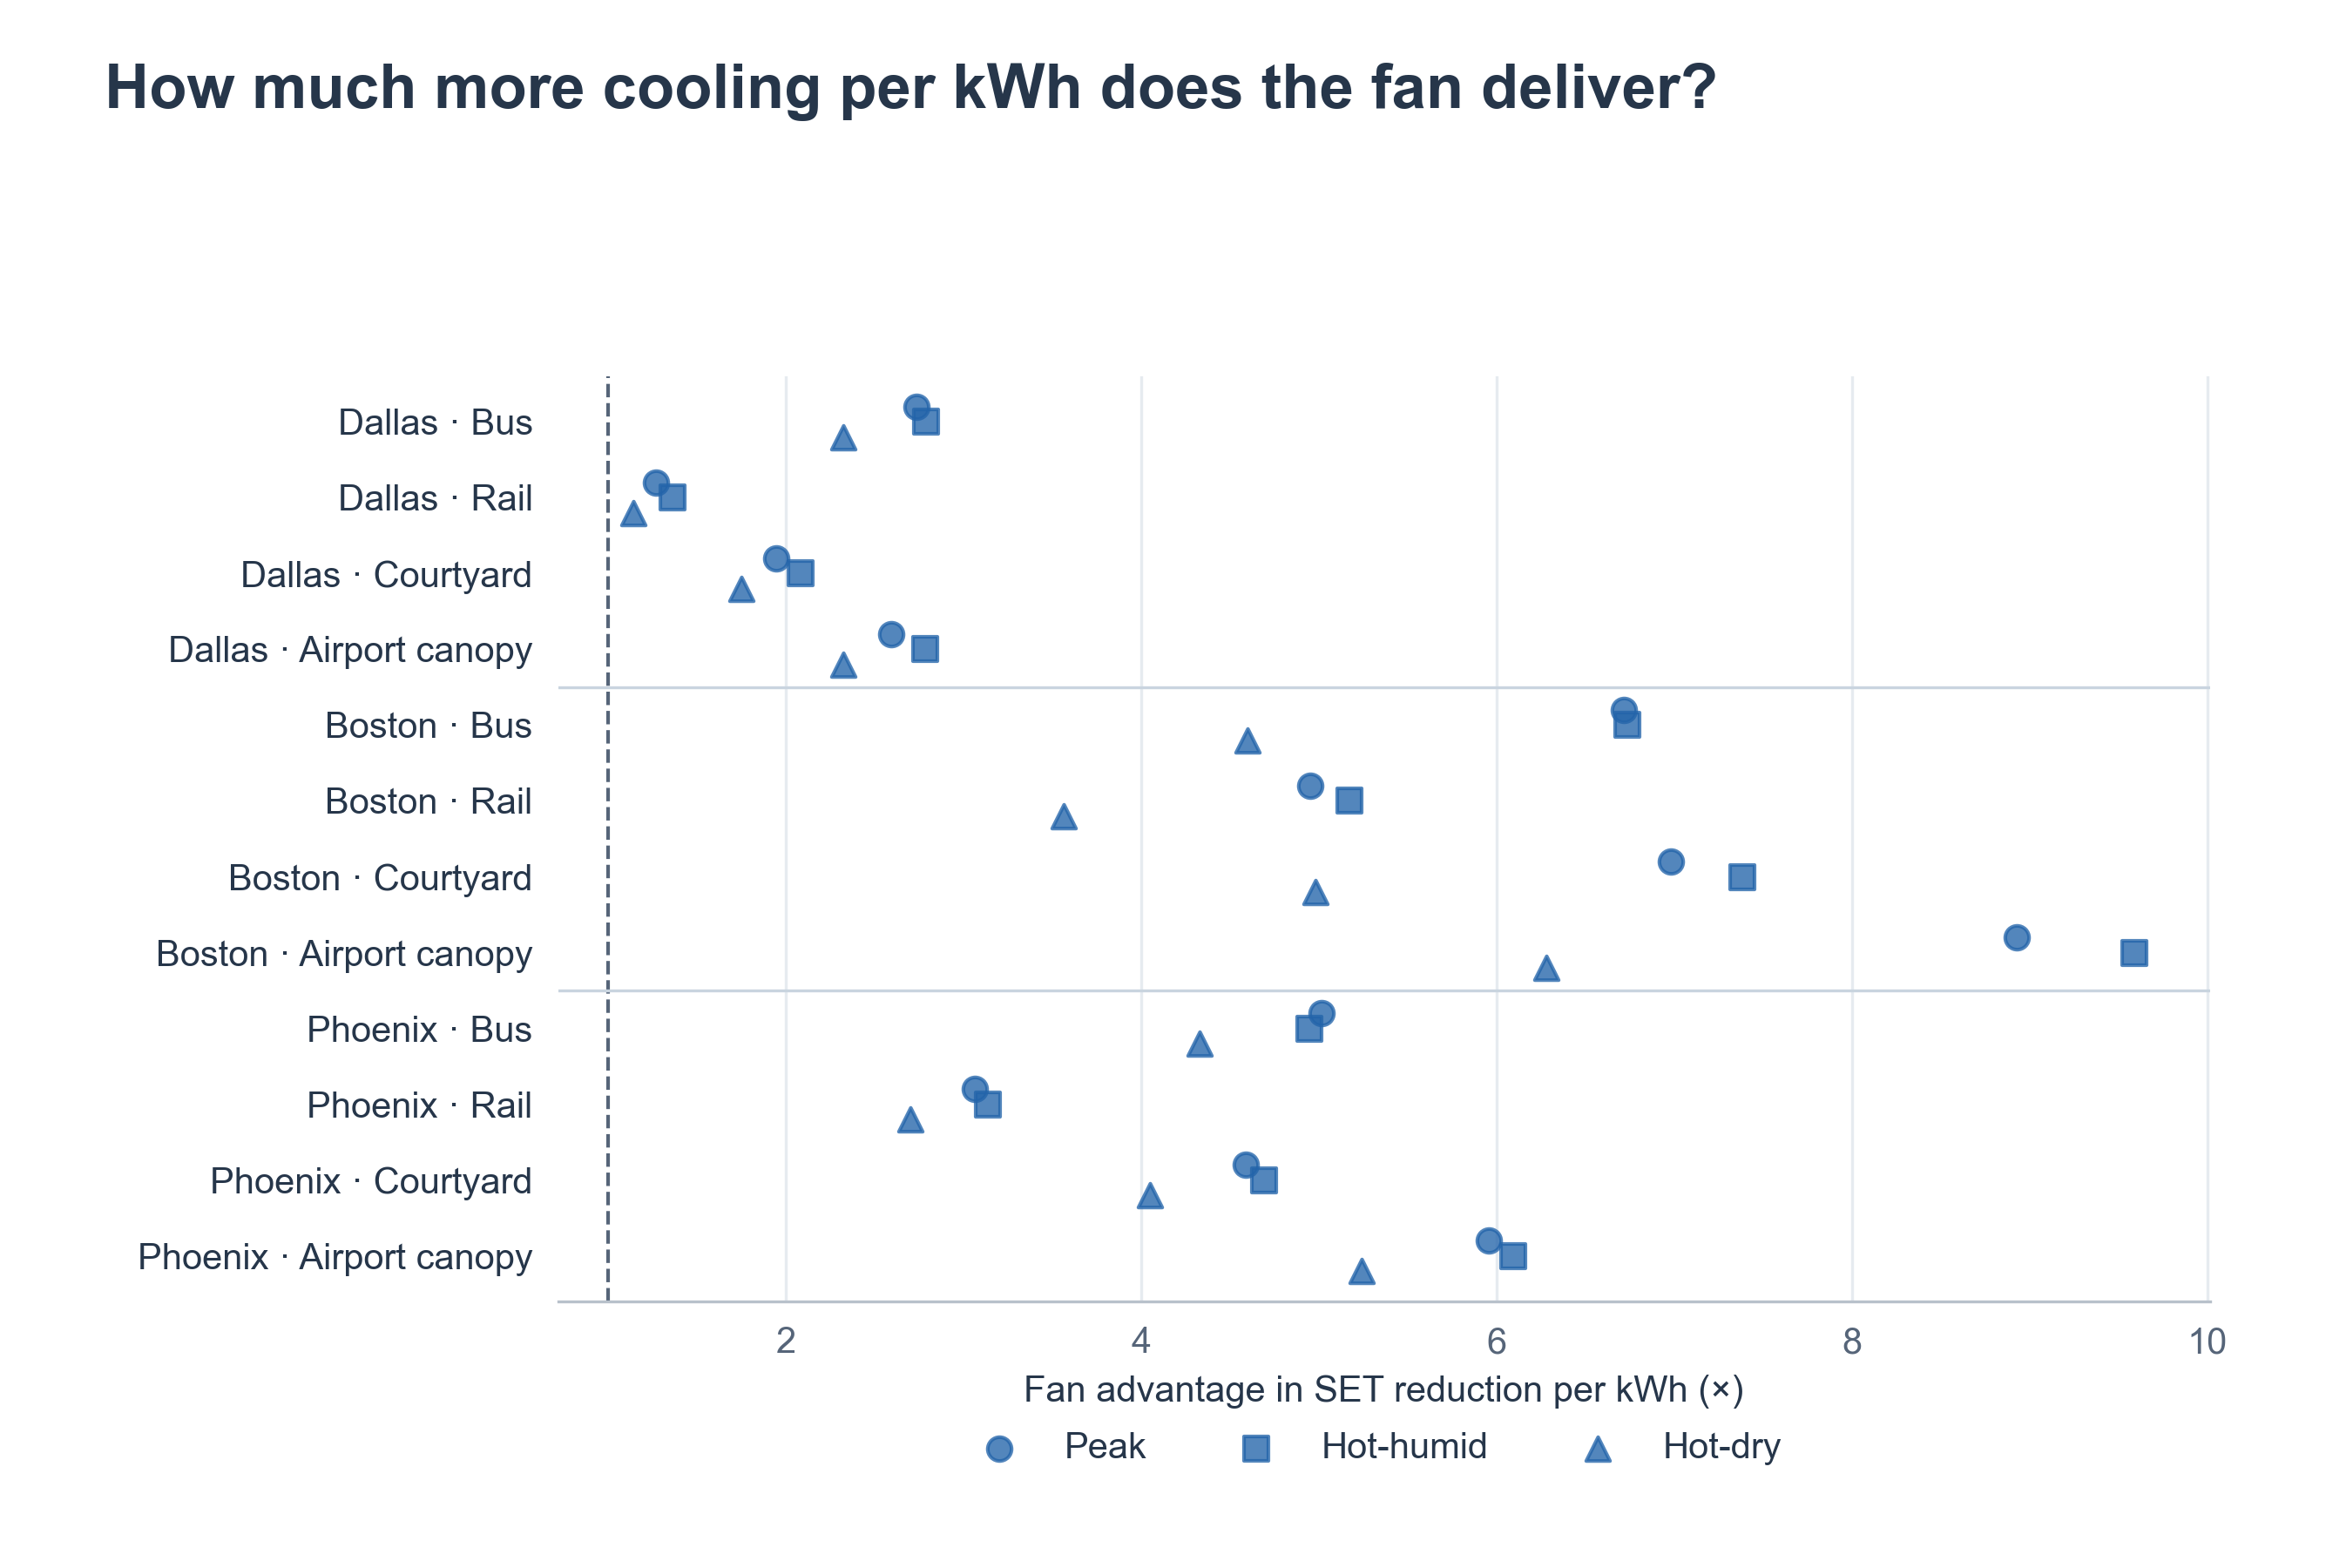
\includegraphics[width=0.66\linewidth]{Images/F12_fan_efficiency_advantage.png}
    \caption{Fan energy efficiency divided by the better evaporative cooler in each case.}
    \label{fig:fan-advantage}
\end{figure}

We used a separate summer-mean reference case to test how outdoor air exchange affects efficiency at the six courtyards and airport canopies. We multiplied the reference exchange rate by two and four while holding the number of devices, their power, and the fan airspeed at the reference person fixed.

\begin{figure}[H]
    \centering
    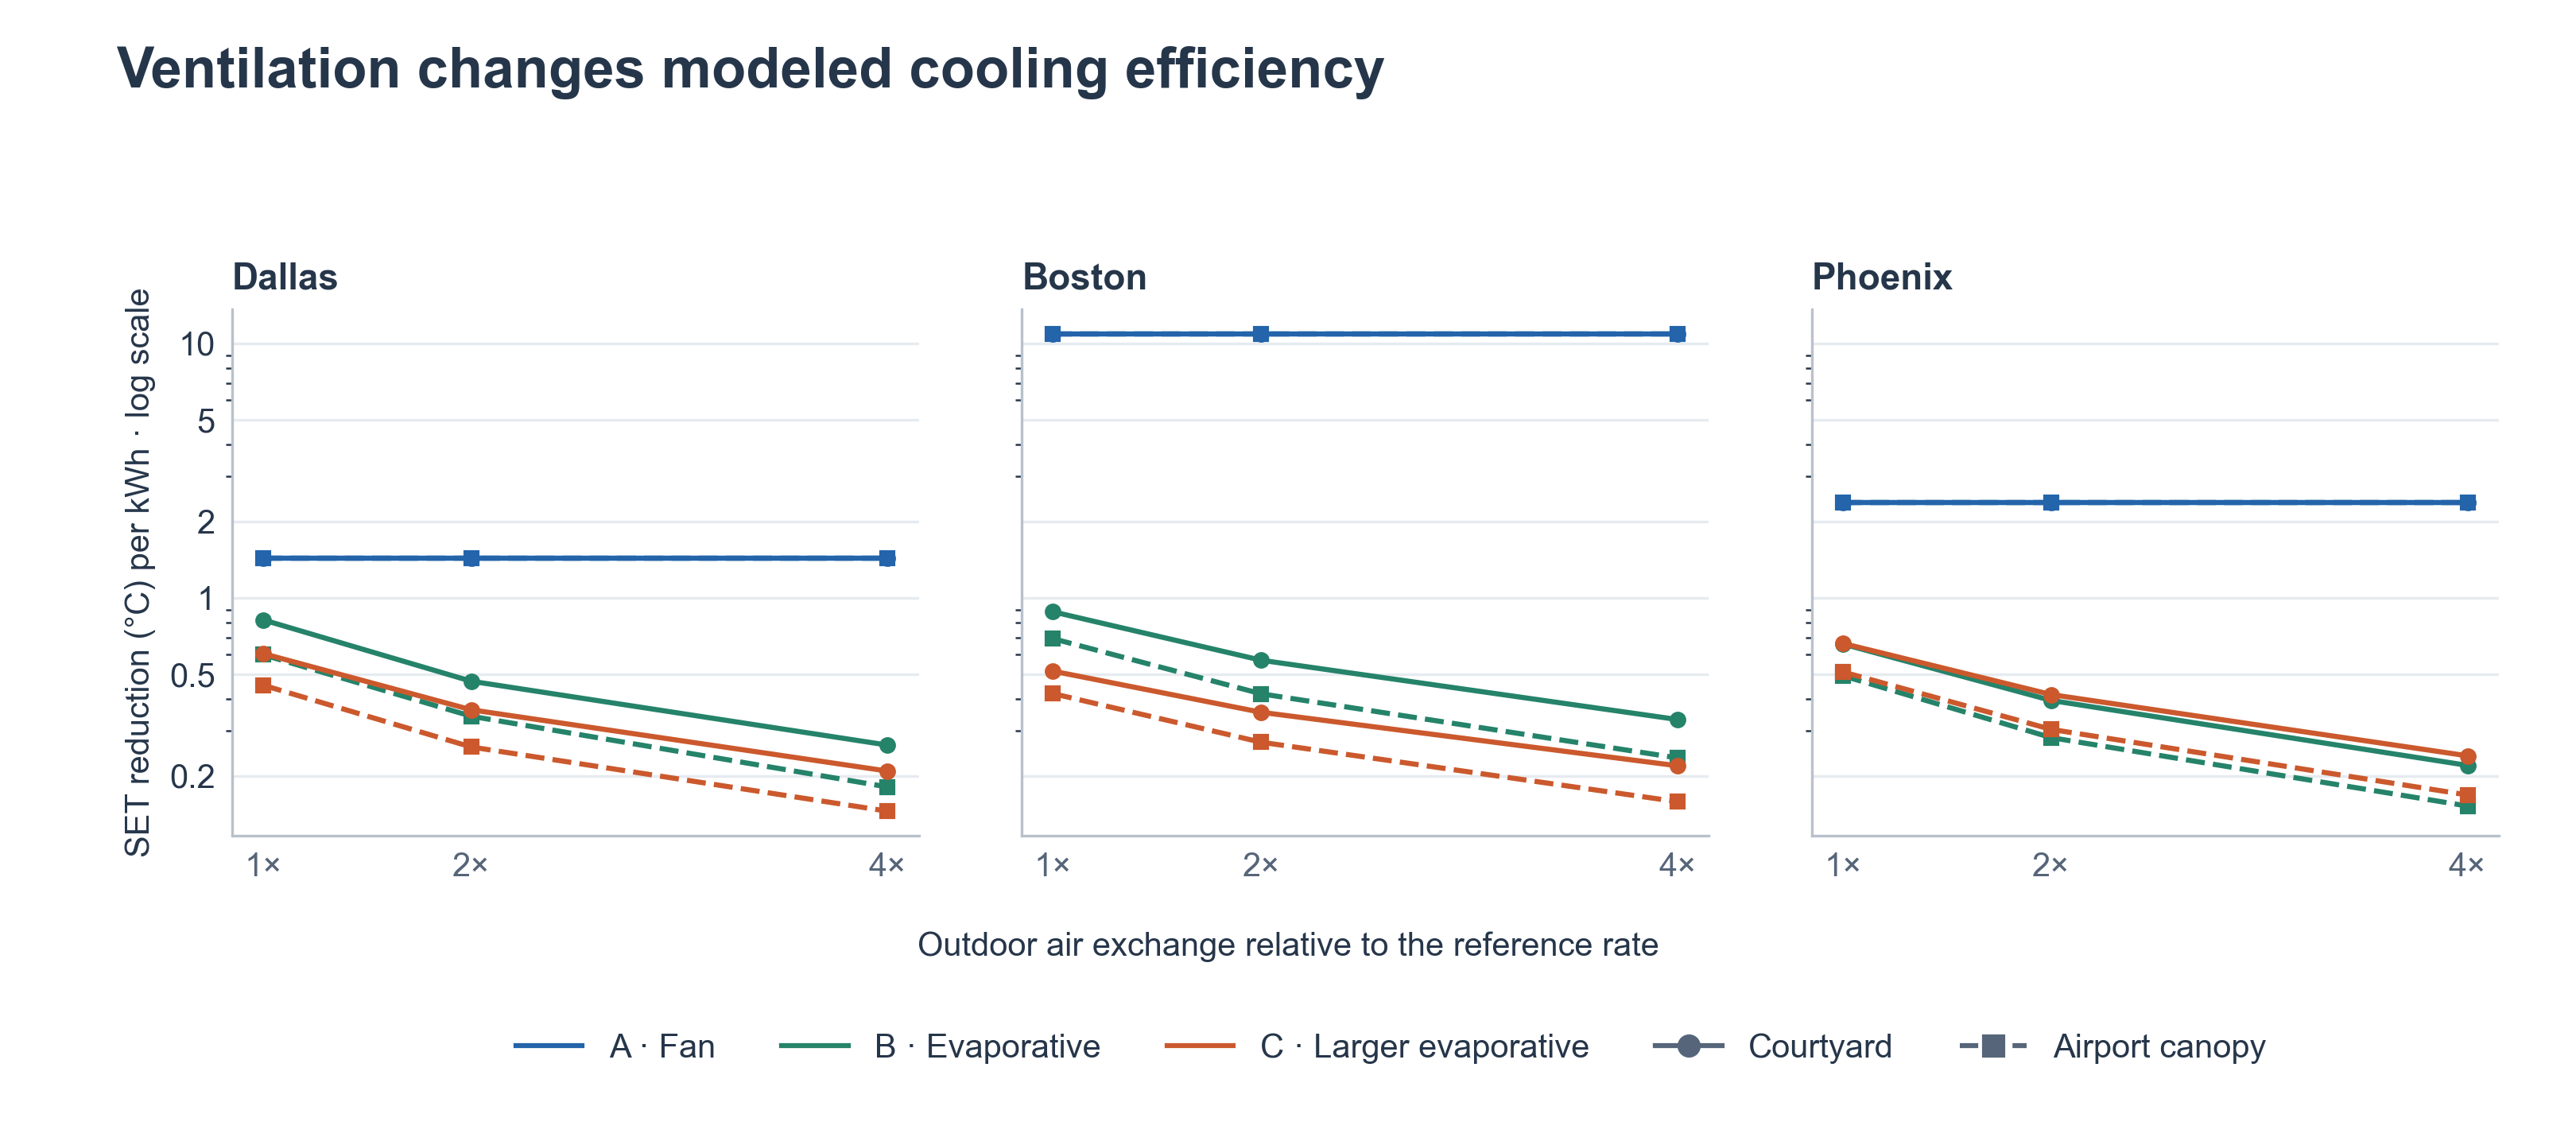
\includegraphics[width=0.9\linewidth]{Images/F11_ventilation_efficiency.png}
    \caption{Cooling efficiency as outdoor air exchange increases. The vertical axis is logarithmic.}
    \label{fig:ventilation-efficiency}
\end{figure}

Evaporative cooling efficiency declined as more outdoor air mixed into the occupied zone. At the Dallas courtyard, quadrupling exchange reduced the larger cooler's SET benefit from 1.51\ensuremath{^{\circ}\mathrm{C}} to 0.52\ensuremath{^{\circ}\mathrm{C}}, a decrease of about 65\%. Its electricity use remained at 2.50 kWh, so its efficiency fell from 0.60 to 0.21\ensuremath{^{\circ}\mathrm{C}} per kWh.

The fan curves are flat because the sweep holds passenger-position airspeed fixed. The courtyard and canopy fan curves overlap within each city because they use the same reference airspeed. The sweep isolates the model's response to exchange and describes a single reference position at each venue.